\section{Q-Learning-Experimente}

Um nun zu testen, ob die Landschaft für unsere Zwecke geeignet ist, werden wir einige Experimente durchführen. Wir wollen hierfür zunächst einen simplen Reinforcement-Learning-Agenten implementieren, welcher \textit{Q-Learning} verwendet.



\subsection{Experimente} \label{sec:qLearningExperiments}
Nachdem der Agent implementiert ist, wollen wir diesen in unserer Umgebung testen. Wir verwenden die zuvor beschriebene Landschaft \ref{img:terrainMain}. Ziel ist es, dass der Agent den höchsten Gipfel erreicht. Zu diesem Zweck liefert die Umgebung als Belohnung die Differenz der Höhe des alten und neuen Zustands. Wenn sich der Agent also von einem Feld mit der Höhe $ 2.3 $ in ein Feld mit der Höhe $ 1.8 $ bewegt erhält er als Belohnung $ -0.5 $.

\paragraph{Einzelnes Experiment}
Nach einigem Ausprobieren haben sich die folgenden Hyperparameter als solche erwiesen, die gute Ergebnisse erzielen:
\begin{minted}{python}
params = Parameters(
            num_episodes=10000,
            max_steps_per_episode=300,
            learning_rate=0.6,
            discount_rate=0.99,
            start_exploration_rate=1,
            max_exploration_rate=1,
            min_exploration_rate=0.01,
            exploration_decay_rate=0.00015,
            # ... Rest wird erst während des Trainigs belegt
        )
\end{minted}

Wir stellen die Ergebnisse in einem Graph da. Nach einem Trainingdurchlauf erhält man die in \ref{img:graphQBest} dargestellte Ausgabe. Die x-Achse stellt die aktuelle Episode dar, während die y-Achse die erhaltene Belohnung, bzw. für die türkise Linie das $ \epsilon $ angibt. Die blaue Linie, welche aufgrund der großen Menge an unterschiedlichen Werten kaum mehr als solche zu erkennen ist, zeigt die Summe der Belohnungen aus allen Zeitschritten für jede Episode an. Die orange Linie ist der Durchschnitt der letzten 100 Gesamtbelohnungen pro Episode. Dieser Wert wird auch als \textit{moving average} bezeichnet. Die Werte von Episode 0 bis 99 sind hier mit 0 belegt. Die türkise Linie zeigt das $ \epsilon $ zu jeder Episode. Die Beschriftung hierfür befindet sich auf der rechten Seite des Graphen.

Es lässt sich an der orangen Linie gut erkennen, wie der Agent mit der Zeit immer bessere Belohnungen erhält.

Lässt man den Agenten nun die im Training erzeugt Q-table verwenden, um die beste Aktion für jeden Zeitschritt auszuwählen, so folgt er dem in \ref{img:pathQBest} sichtbaren Pfad. Er findet also den höchsten Berg in der gegebenen Landschaft, obwohl dieser weit entfernt vom Startpunkt in der Mitte und hinter einem Graben liegt.

\begin{figure}[H]
    \centering
    \begin{subfigure}[b]{0.49\textwidth}
        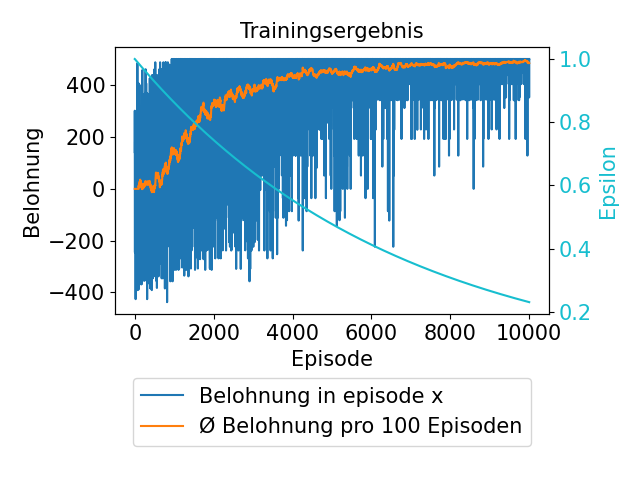
\includegraphics[width=\textwidth]{q_learning/figure_best.png}
        \caption{x-Achse zeigt die Episode, y-Achse zeigt die Belohnung. Eingezeichnet sind exakte Belohnung (blau), deren moving average (orange) und der Wert von $ \epsilon $ (türkis, Achse rechts) pro Episode.}
        \label{img:graphQBest}
    \end{subfigure}
    \begin{subfigure}[b]{0.49\textwidth}
        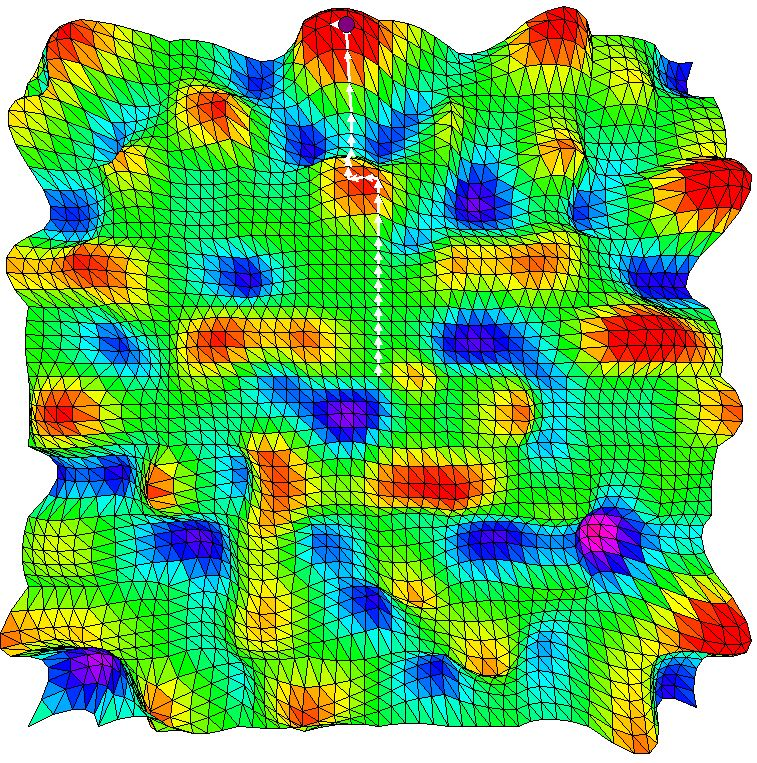
\includegraphics[width=\textwidth]{q_learning/terrain_path_best_white_3.JPG}
        \caption{Bester Pfad des Agenten nach dem Training}
        \label{img:pathQBest}
    \end{subfigure}
    \caption{Trainingsergebnisse des ersten Experiments}
\end{figure}

Eine weiter interessanter Wert ist die Anzahl der mit 0 belegten Einträge in der Q-table. Diese besitzen entweder zufällig den errechneten Q-value 0 oder wurden vom Agenten nicht berechnet. Da die meisten Einträge im 14-Stelligen Nachkommabereich liegen, ist ersteres relativ unwahrscheinlich und so lässt sich sagen, dass die Summe der mit 0 belegten Einträge ungefähr der Summe der nicht erkundeten Zustände entspricht. In Fall des aktuellen Experiments sind 850 der 10000 Einträge mit 0 belegt. Der Agent hat also ungefähr $ 91.5\% $ der Umgebung erkundet.

Dies ist nur ein einzelnes Experiment und hat natürlich keine statistische Aussagekraft. Es diente lediglich der Demonstration und der Erklärung der Visualisierung. Wir werden im Folgenden testen, welche Auswirkung die Verwendung der $ \epsilon $-greedy Strategie auf den Lernprozess hat.

\paragraph{Vergleich des Trainings mit und ohne $ \epsilon $-greedy Strategie}
Um eine aussagenkräftigere Datengrundlage zu erhalten, werden wir die folgenden Experimente jeweils 20 mal wiederholen. Diese Zahl hat sich als ein gutes Mittelmaß zwischen einer ausreichenden Menge an Daten für die Statistik und der Berechenbarkeit in zumutbarer Zeit erwiesen.

Die erste Experimentreihe erfolgt mit den gleichen Parametern wie im vorherigen Experiment. Für die zweite Experimentreihe setzen wir lediglich $ \epsilon $ auf 0. Das kommt dem Weglassen der $ \epsilon $-greedy Strategie gleich und bedeutet, dass der Agent in jedem Fall greedy agiert und die beste Aktion wählt. Dies soll die Notwendigkeit von $ \epsilon $ für ein besseres Trainingsergebnis zeigen.
\begin{figure}[H]
    \centering
    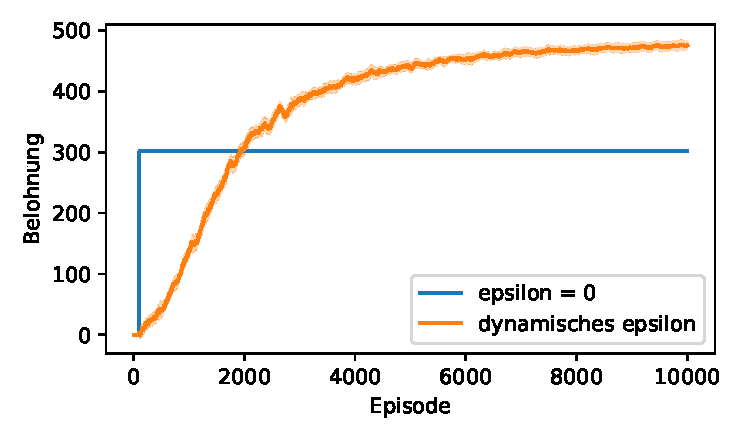
\includegraphics{q_learning/figure_epsilon_compare.pdf}
    \caption{Vergleich der Trainingsverläufe mit und ohne $ \epsilon $-greedy Strategie nach jeweils 20 Wiederholungen. Der Graph zeigt den moving average und dessen Standardabweichung pro Episode.} \label{img:graphQEpsComp}
\end{figure}
Die Achsen von Graph \ref{img:graphQEpsComp} sind bis auf das Fehlen der $ \epsilon $-Achse identisch mit dem aus \ref{img:graphQBest}. Die beiden Linien zeigen jeweils den Durchschnitt der moving average Werte aller 20 Experimentiterationen. Der leicht transparente Bereich um die Linien herum ist die Standartabweichung in der jeweiligen Episode.
Es lässt sich hier sehr deutlich erkennen, dass der Agent ohne eine Erkundungsstrategie wie $ \epsilon $-greedy (blaue Linie) zu Beginn einen relativ lukrativen Pfad findet, diesen aber dann auch nicht mehr verlässt, um andere Pfade zu erkunden und so immer die gleiche Belohnung bekommt. Er wird schließlich vom $ \epsilon $-greedy Agenten (orange Linie) überholt, da dieser seine Umgebung erkundet. Dieser erhält am Ende des Trainings wesentlich höhere Belohnungen.

Betrachten wir den Durchschnitt der Anzahl der mit 0 belegten Einträge der Q-tables beider Experimentreihen lässt sich abschätzen, dass der $ \epsilon $-greedy Agent im Schnitt $ 89.9\% $ der Umgebung erkundet hat, während es beim Agent ohne Erkundungsstrategie gerade einmal $ 1.1\% $ sind.

Dies zeigt, dass eine Erkundungsstrategie für den Erfolg des Agenten sehr wichtig ist.

\paragraph{Erkundungsstrategie codiert im Reward}
Für das nächste Experiment lassen wir der Agenten ebenfalls in jedem Zeitschritt greedy agieren. Diesmal erreichen wir dies, indem wir unabhängig vom aktuellen $ \epsilon $ immer die beste Aktion auswählen. Der Agent soll allein durch die Veränderung der Belohnung dazu gebracht werden, seine Umgebung besser zu erkunden und trotzdem einen möglichst hohen Punkt zu finden.

Wir modifizieren hierfür die nach jeder Aktion von der Umgebung erhaltene Belohnung wiefolgt:
\begin{minted}{python}
new_state, actual_reward, _ = environment.agent_perform_action(action)

reward = ((1 - exploration_rate) * actual_reward) - exploration_rate

sars = (state, action, reward, new_state)
buffer.append(sars)
\end{minted}
Die \mintinline{python}{exploration_rate} verhält sich hierbei genau so wie beim Experiment davor. Diese Formel soll bewirken, dass der Agent zu Beginn bei einer hohen \mintinline{python}{exploration_rate} alle besuchten Felder mit einem negativen Wert belegt, sodass er beim nächsten mal andere Felder besucht und so seine Umgebung erkundet. Nach und nach wird diese Belegung dann immer mehr mit den mittels korrekter Belohnungen ermittelten Q-values ersetzt, wodurch sich der Agent auf die besten Zustände einpendeln soll. Wir setzen die learning rate auf 1, damit der Agent nicht an den zu Beginn verfälschten Belohnungen festhält. Nach 50000 Episoden erhält man folgendes Ergebnis:
\begin{figure}[H]
    \centering
    \begin{subfigure}[b]{0.49\textwidth}
        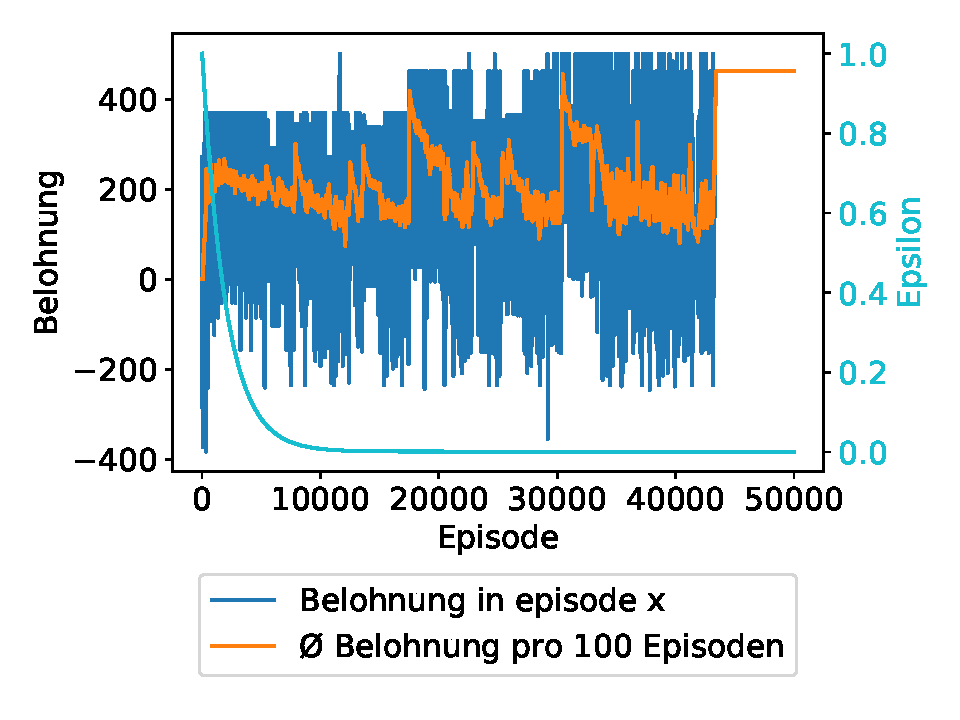
\includegraphics[width=\textwidth]{q_learning/figure_epsilon_in_reward_2.pdf}
        \caption{Graph so wie in \ref{img:graphQBest}}
        \label{img:graphQEpsInRew}
    \end{subfigure}
    \begin{subfigure}[b]{0.49\textwidth}
        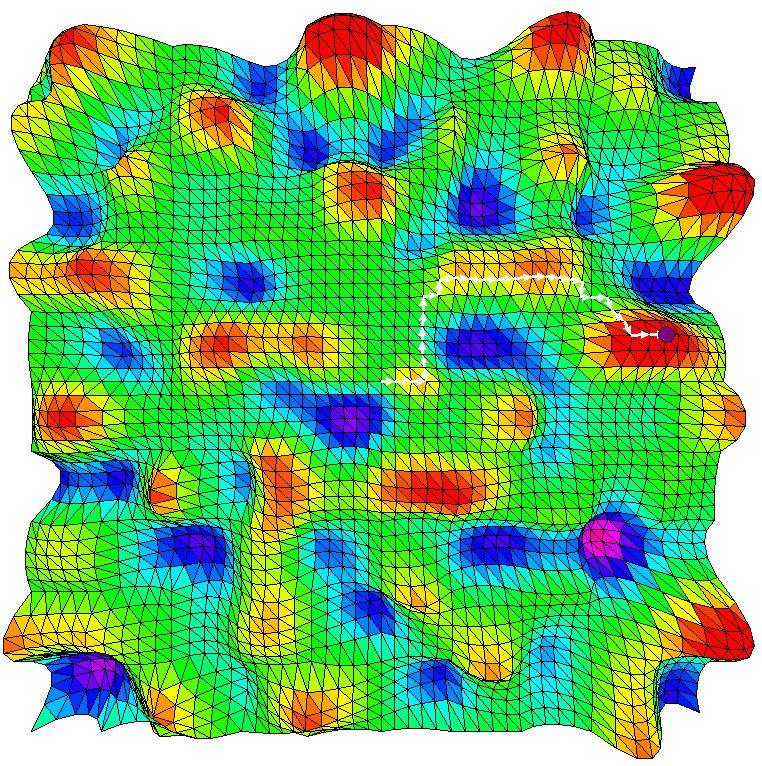
\includegraphics[width=\textwidth]{q_learning/terrain_epsilon_in_reward.JPG}
        \caption{Bester Pfad des Agenten nach dem Training}
        \label{img:pathQEpsInRew}
    \end{subfigure}
    \caption{Trainingsergebnisse mit Erkundungsstrategie codiert im Reward}
\end{figure}
Wichtig ist es an dieser Stelle zu erwähnen, dass der Graph \ref{img:graphQEpsInRew} die unverfälschte, von der Umgebung gelieferte Belohnung vor der Modifikation zeigt, da uns der tatsächliche Lernfortschritt des Agenten interessiert und man diesen sonst nicht mit den Ergebnissen anderen Experimente vergleichen könnte. Es fällt deutlich auf, dass der Lernprozess hier anders verläuft als in \ref{img:graphQBest}. Wir erhalten keine saubere Lernkurve. Trotzdem erreicht der Agent einen maximalen moving average von etwas über 462. Zum Vergleich: Der maximale moving average von \ref{img:graphQBest} liegt bei etwas über 497. Die Q-table dieses Experiments enthält 850 von 10000 mit Null belegte Einträge.

Abbildung \ref{img:pathQEpsInRew} zeigt den Pfad des Agenten bei Verwendung der erzeugten Q-table. Er findet zwar nicht den höchsten Punkt, erklimmt aber dennoch einen hohen Berg, welcher sich nicht in unmittelbarer Nähe des Startzustands befindet. Die Strategie hat also zur besseren Erkundung der Umgebung beigetragen.

Wiederholt man das Experiment 20 mal, so lässt sich der folgende Durchschnitt mit Standartabweichung berechnen:
\begin{figure}[H]
    \centering
    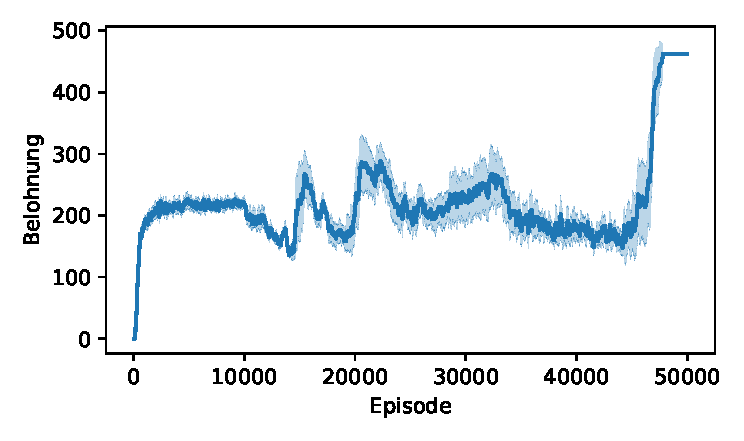
\includegraphics{q_learning/figure_epsilon_in_reward_mean.pdf}
    \caption{Trainingsergebnisse mit Erkundungsstrategie codiert im Reward nach 20 Wiederholungen. Graph so wie in \ref{img:graphQEpsComp}.} \label{img:graphQEpsInRewMean}
\end{figure}
Der Agent benötigt mit 50000 Episoden sehr lange, um seinen Höchstwert zu erreichen. Dieser scheint sich auch nach circa Episode 47 nicht mehr zu verändern, was vermutlich darauf zurückzuführen ist, dass der Agent immer greedy agiert und zu diesem Zeitpunkt kein besserer ihm bekannter Pfad mehr existiert. Verglichen mit dem Agenten ohne Erkundungsstrategie lässt sich festhalten, dass die Modifikation der Belohnung in diesem Fall eine höheren Ertrag sowie eine bessere Erkundung der Umgebung bewirkt hat. Diese Strategie dauert allerdings deutlich länger und liefert etwas weniger Ertrag als die klassische $ \epsilon $-greedy Strategie.
% \begin{minted}{python}
% params = Parameters(
%         num_episodes=100,
%         max_steps_per_episode=20,

%         learning_rate=0.5,
%         discount_rate=0.99,

%         start_exploration_rate=1,
%         max_exploration_rate=1,
%         min_exploration_rate=0.01,
%         exploration_decay_rate=0.1,

%         rewards_all_episodes=[],
%         max_rewards_all_episodes=[],
%     )
% \end{minted}

% https://github.com/simoninithomas/Deep_reinforcement_learning_Course/tree/master/Q%20learning/FrozenLake

% \begin{figure}[h]
%     \centering
%     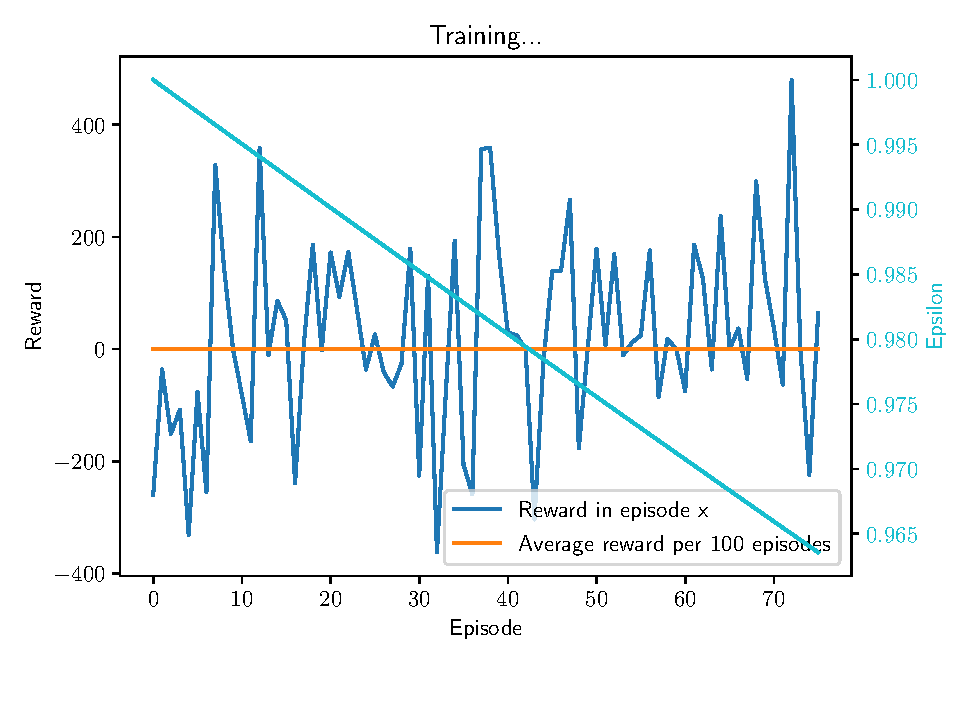
\includegraphics[width=\textwidth]{plot_test.pdf}
%     \caption{Visualisierung von zweidimensionaler Perlin Noise} \label{img:terrainMain}
% \end{figure}

% \begin{align}
%     \mathcal{F}(\theta) & = H(A|S,Z) - H(Z|S) + H(Z) \nonumber\\
%     & = H(A|S,Z) + E_{z \sim p(z), s \sim \pi(z)}(log\ p(z | s)) - E_{z \sim p(z)}(log\ p(z)) \label{eq:objective_2}\\
%     & \ge H(A|S,Z) + E_{z \sim p(z), s \sim \pi(z)}(log\ q_\phi(z | s) - log\ p(z)) \stackrel{\triangle}{=} \mathcal{G}(\theta, \phi) \nonumber
% \end{align}


% Grid, auf dem sich der Agent bewegen
% Perlin Noise
% 
% Color-coded: Rot ist hoch, blau ist tief
% 

%% Ziel des Agenten

%% Agent mit Q-Table

%% Agent mit Neuronalem Netz

%% Ergebnisse

% \begin{minted}{python}
%     import numpy as np
      
%     def incmatrix(genl1,genl2):
%         m = len(genl1)
%         n = len(genl2)
%         M = None #to become the incidence matrix
%         VT = np.zeros((n*m,1), int)  #dummy variable
      
%         #compute the bitwise xor matrix
%         M1 = bitxormatrix(genl1)
%         M2 = np.triu(bitxormatrix(genl2),1) 
      
%         for i in range(m-1):
%             for j in range(i+1, m):
%                 [r,c] = np.where(M2 == M1[i,j])
%                 for k in range(len(r)):
%                     VT[(i)*n + r[k]] = 1;
%                     VT[(i)*n + c[k]] = 1;
%                     VT[(j)*n + r[k]] = 1;
%                     VT[(j)*n + c[k]] = 1;
      
%                     if M is None:
%                         M = np.copy(VT)
%                     else:
%                         M = np.concatenate((M, VT), 1)
      
%                     VT = np.zeros((n*m,1), int)
      
%         return M
%     \end{minted}